\documentclass{IEEEtran}
\usepackage{filecontents}
\usepackage{lipsum}
\usepackage[utf8]{inputenc}
\usepackage{graphicx} % for image
\usepackage{color} % for image (?)
\usepackage{amsmath}
\usepackage{tikz}
\usetikzlibrary{shapes.gates.logic.US,trees,positioning,arrows}

% correct bad hyphenation here
\hyphenation{op-tical net-works semi-conduc-tor}


\begin{document}

\title{SSA\\Otimização do perfil de tensão em Linhas de Distribuição de Energia por Injeção de Potência reativa via um Algoritmo Evolucionário Denominado \textit{Particle Swarm Optimization}}
%
%
% author names and IEEE memberships
% note positions of commas and nonbreaking spaces ( ~ ) LaTeX will not break
% a structure at a ~ so this keeps an author's name from being broken across
% two lines.
% use \thanks{} to gain access to the first footnote area
% a separate \thanks must be used for each paragraph as LaTeX2e's \thanks
% was not built to handle multiple paragraphs
%

\author{Luiz~Le~Roy - ~\IEEEmembership{PUC Minas}
        % <-this % stops a space
\thanks{Texto iniciado em 4 de abril de 2014.}}

% The paper headers
\markboth{Journal of \LaTeX\,~Vol.~X, No.~Y, Abril~2014}%
{Shell \MakeLowercase{\textit{et al.}}: Bare Demo of IEEEtran.cls for Journals}

% make the title area
\maketitle

\begin{abstract}
Os objetivos principais estão relacionados com a alocação de capacitores em sistemas de média e alta tensão. Os bancos de capacitores em paralelo (shunt) são largamente utilizados principalmente nos alimentadores primários dos sistemas de distribuição e em subestações para compensar a deficiência de potência reativa e, consequentemente, obter melhores perfis de tensão, reduções das perdas de potência e energia, e aumento da capacidade em atender carga ativa. No entanto, as instalações de capacitores em locais impróprios aumentam os níveis de tensão inadequados, elevando as demandas das cargas, consequentemente, aumentando as perdas globais do sistema.
A determinação do local ótimo de instalação de bancos de capacitores corresponde a um problema de programação matemática combinatorial e engloba a escolha da localização, o tamanho e quantidade de bancos de capacitores a serem instalados no sistema. Nesta avaliação, deve-se realizar uma análise econômica que reflete a eficiência dos investimentos de capital (Ex.: aquisição, custo de instalação, custos de operação e manutenção, perdas, etc.) e dos benefícios com a melhoria do perfil de tensão.
O controle de tensão através de alocação de potência reativa é alvo de intensa investigação, sendo as primeiras publicações na década de 50. No entanto, pode-se considerá-lo um tema bastante atual devido às condições críticas em que se encontra a operação dos Sistemas Elétricos de Potência (SEP), estando próximos de seus limites operacionais, além dos recursos que estão se esgotando devido ao retardo de investimentos.

\end{abstract}

\begin{IEEEkeywords}
PSO \textit{(Particle Swarm Optimization)}.
\end{IEEEkeywords}

\IEEEpeerreviewmaketitle

\section{Introdução}
\IEEEPARstart{A}{pós} conversar com o orientador fizemos o seguinte combinado:
Devemos concentrar em duas diretivas:
\begin{itemize}[]
\item Buscar um problema de maior ganho para a Cemig, e
\item encontrar algo que pode trazer ganhos para concessionárias de energia de forma geral.
\end{itemize}

No primeiro caso, podemos tentar encontrar uma contribuição dentro de uma realidade nacional, que possui diversas peculiaridades. No segundo item, podemos abordar mais as inúmeras possibilidades de contribuições científicas.

\section{Bibliografia Preliminar}
PSO para SEP: \textit{Particle Swarm Optimization}.
Paralelismo:

\section{{Organogramas}
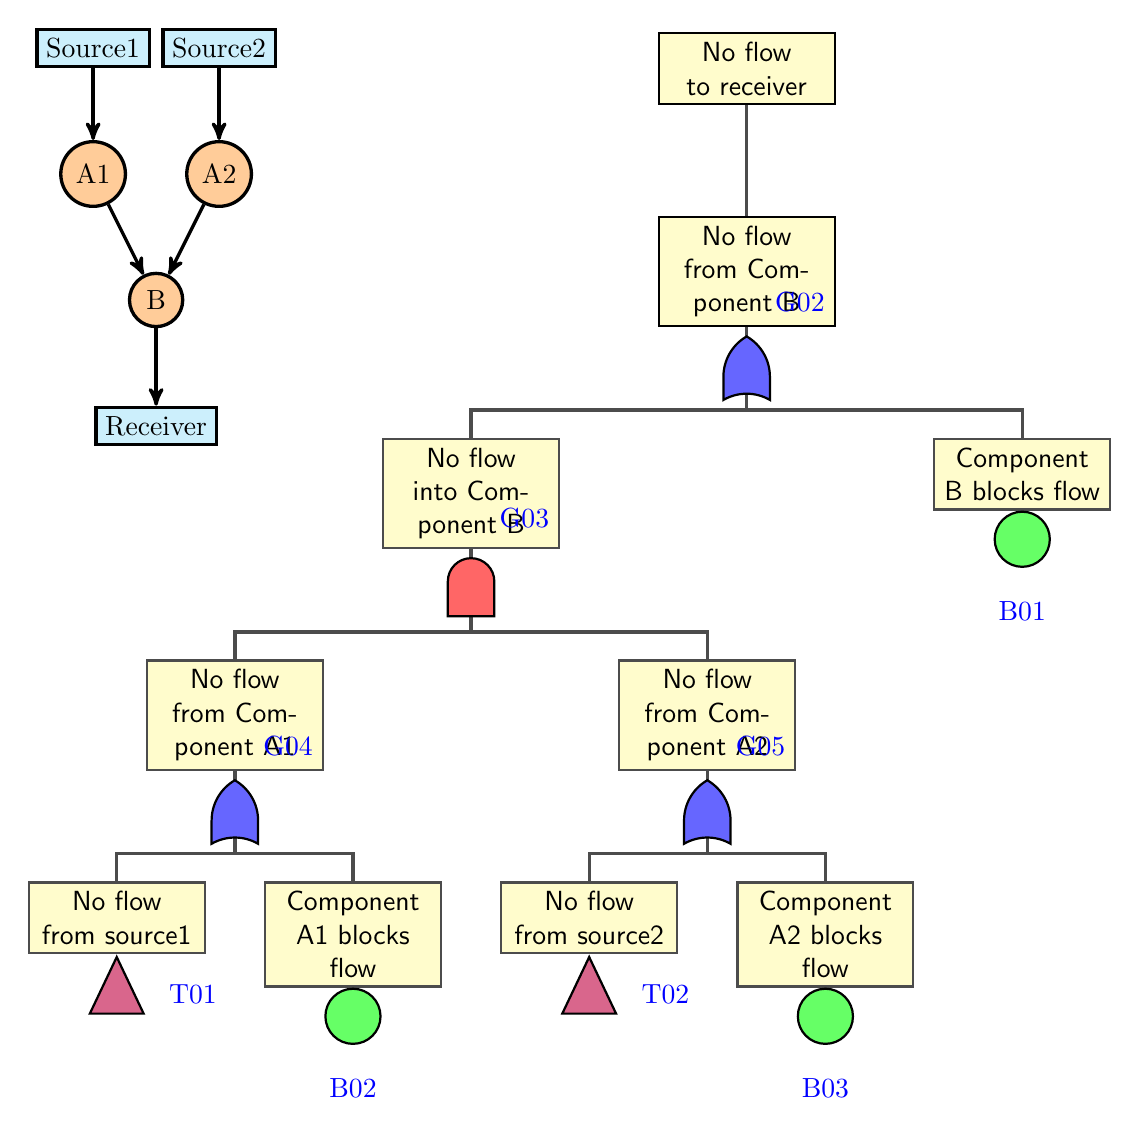
\begin{tikzpicture}[
% Gates and symbols style
    and/.style={and gate US,thick,draw,fill=red!60,rotate=90,
		anchor=east,xshift=-1mm},
    or/.style={or gate US,thick,draw,fill=blue!60,rotate=90,
		anchor=east,xshift=-1mm},
    be/.style={circle,thick,draw,fill=green!60,anchor=north,
		minimum width=0.7cm},
    tr/.style={buffer gate US,thick,draw,fill=purple!60,rotate=90,
		anchor=east,minimum width=0.8cm},
% Label style
    label distance=3mm,
    every label/.style={blue},
% Event style
    event/.style={rectangle,thick,draw,fill=yellow!20,text width=2cm,
		text centered,font=\sffamily,anchor=north},
% Children and edges style
    edge from parent/.style={very thick,draw=black!70},
    edge from parent path={(\tikzparentnode.south) -- ++(0,-1.05cm)
			-| (\tikzchildnode.north)},
    level 1/.style={sibling distance=7cm,level distance=1.4cm,
			growth parent anchor=south,nodes=event},
    level 2/.style={sibling distance=7cm},
    level 3/.style={sibling distance=6cm},
    level 4/.style={sibling distance=3cm}
%%  For compatability with PGF CVS add the absolute option:
%   absolute
    ]
%% Draw events and edges
    \node (g1) [event] {No flow to receiver}
	     child{node (g2) {No flow from Component B}   
	     	child {node (g3) {No flow into Component B}
	     	   child {node (g4) {No flow from Component A1}
	     	      child {node (t1) {No flow from source1}}
	     	      child {node (b2) {Component A1 blocks flow}}
			}
	     	   child {node (g5) {No flow from Component A2}
	     	      child {node (t2) {No flow from source2}}
	     	      child {node (b3) {Component A2 blocks flow}}
			}
		   }
	     	child {node (b1) {Component B blocks flow}}
		};
%% Place gates and other symbols
%% In the CVS version of PGF labels are placed differently than in PGF 2.0
%% To render them correctly replace '-20' with 'right' and add the 'absolute'
%% option to the tikzpicture environment. The absolute option makes the 
%% node labels ignore the rotation of the parent node. 
   \node [or]	at (g2.south)	[label=-20:G02]	{};
   \node [and]	at (g3.south)	[label=-20:G03]	{};
   \node [or]	at (g4.south)	[label=-20:G04]	{};
   \node [or]	at (g5.south)	[label=-20:G05]	{};
   \node [be]	at (b1.south)	[label=below:B01]	{};
   \node [be]	at (b2.south)	[label=below:B02]	{};
   \node [be]	at (b3.south)	[label=below:B03]	{};
   \node [tr]	at (t1.south)	[label=below:T01]	{};
   \node [tr]	at (t2.south)	[label=below:T02]	{};
%% Draw system flow diagram
   \begin{scope}[xshift=-7.5cm,yshift=-5cm,very thick,
		node distance=1.6cm,on grid,>=stealth',
		block/.style={rectangle,draw,fill=cyan!20},
		comp/.style={circle,draw,fill=orange!40}]
   \node [block] (re)					{Receiver};
   \node [comp]	 (cb)	[above=of re]			{B}  edge [->] (re);
   \node [comp]	 (ca1)	[above=of cb,xshift=-0.8cm]	{A1} edge [->] (cb);
   \node [comp]	 (ca2)	[right=of ca1]			{A2} edge [->] (cb);
   \node [block] (s1)	[above=of ca1]		{Source1} edge [->] (ca1);
   \node [block] (s2)	[right=of s1]		{Source2} edge [->] (ca2);
   \end{scope}
\end{tikzpicture}

\section{Conclusão}
Até o momento, foi possível concluir coisas interessantes sobre a alocação estática de dispositivos capacitivos em linhas de distribuição:

By Luiz Le Roy et. al.: \cite{arruda2005calculation}, \cite{adriano2006modelos} e \cite{adriano2006efeitos}.



% Can use something like this to put references on a page
% by themselves when using endfloat and the captionsoff option.
\ifCLASSOPTIONcaptionsoff
  \newpage
\fi

\bibliographystyle{ieeetran}
\bibliography{bibliography}

\begin{IEEEbiographynophoto}{Luiz~Le~Roy}
é estudante do curso de mestrado da Pontif\'icia Universidade Cat\'olica de Minas Gerais.
\end{IEEEbiographynophoto}

% that's all folks
\end{document}
